\chapter{Server configuration}

\section{Security}

To protect our server, we had to setting up some security systems. A lot of these attacks consists to login on some sensitive services: \textit{SSH}, \textit{Asterisk}, \textit{FTP}... And our server didn't escape to these attacks. 

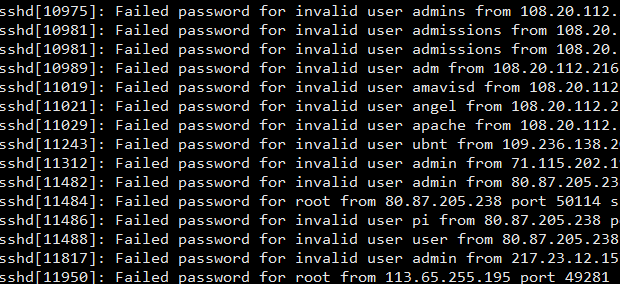
\includegraphics[width=1\textwidth]{img/sshattacks.png}

\subsection{Firewall}

For a simple protection, we generated some firewall rules to allows the inbound port we need. For this project, we needed this following ports list:
\begin{itemize}
\item \textit{SIP}: 5060-5082 (TCP/UDP)	
\item \textit{RTP}: 10000-20000 (UDP)
\item \textit{MySQL}: 3306 (TCP)
\item \textit{SSH}: 22 (TCP)
\item \textit{WEB}: 80,443 (TCP)
\item \textit{DNS}: 53 
\item \textit{PING}: ICMP
\end{itemize}

\subsection{fail2ban}
As said previously, our server has been often attacked. To prevent these attacks by brute-force, we installed the software \textit{fail2ban}. Once installed, it begins to read logs files and blocks suspicious IP for few minutes. Highly customizable, it natively supports a lot of services as \textit{SSH}, \textit{FTP} and \textit{Asterisk}! 
When an IP is blocked, it stays blocked for few minutes, then it is removed from the ban list. If this IP is caught again, it is definitively blocked.


\section{A reverse proxy, Nginx}

By default, Tomcat is running on port \textbf{8080}, so it isn't the default HTTP port which is \textbf{80}. Because all ports under \textit{1024} are reserved to \textit{root} user, we chose to not launch the tomcat server as \textit{root} user to prevent some attacks. In this way, we installed a reverse proxy on the port 80. As reverse proxy, we used the \textbf{Nginx} server.
Because \textbf{Nginx} only redirect the incoming traffic through the internal network to the \textbf{Tomcat} server, it is impossible for the web application to access sensitive data in the system.

\section{MySQL, different users}
Parler ici des differents utilisateurs pour le site et pour le nodeJS.

